% =====================================================================
% 6.3 Estabilidade e fator de qualidade
% =====================================================================
\subsection{Estabilidade e fator de qualidade}

A Tabela~\ref{tab:hestab} traz o maior passo estável de cada método, calculado pela função \(R(z)\) da Equação~\eqref{eq:Rz} com os autovalores do circuito. No Euler, o valor coincide com \(RC\), como prevê a Equação~\eqref{eq:heuler}: 20,0~\(\mu\)s com \(Q=5\) e 2,00~\(\mu\)s com \(Q=50\). Quando \(Q\) aumenta dez vezes, o limite do Euler cai dez vezes, e o do RK4 quase não muda.

\begin{table}[htbp]
\centering
\caption{Maior passo absolutamente estável de cada método.}
\label{tab:hestab}
\small
\begin{tabular}{@{}lrrr@{}}
\toprule
Circuito & Euler & Euler melhorado & RK4 \\
\midrule
\(R=20~\Omega\), \(Q=5\) & 20{,}0~\(\mu\)s & 104{,}9~\(\mu\)s & 295{,}0~\(\mu\)s \\
\(R=2~\Omega\), \(Q=50\) & 2{,}00~\(\mu\)s & 44{,}4~\(\mu\)s & 284{,}8~\(\mu\)s \\
\bottomrule
\end{tabular}
\fonte{Elaborado pelos autores (2026).}
\end{table}

O período natural do circuito é \(2\pi/\omega_0\approx 628~\mu\mathrm{s}\). Com \(Q=50\), o Euler precisa de mais de trezentos passos por período só para não divergir. O RK4 continua estável com pouco mais de dois passos por período, embora com erro grande. Estabilidade não é precisão. Ela é a condição mínima para que a precisão possa ser discutida.

A Figura~\ref{fig:estab} confere essa previsão na prática. Ela integra o degrau até 6~ms e marca o pico de \(|i|\) para cada passo. As retas verticais são os limites da Tabela~\ref{tab:hestab}. Com \(Q=5\), o pico físico fica perto de 43~mA. Com \(h=25~\mu\mathrm{s}\), acima do limite, o Euler já chega a 0,21~A. Com \(h=40~\mu\mathrm{s}\), a integração para por divergência. O Euler melhorado continua físico até 80~\(\mu\)s (pico de 45~mA) e chega a 1,10~A em 120~\(\mu\)s. O RK4 com \(h\approx 286~\mu\mathrm{s}\), ainda abaixo do limite de 295~\(\mu\)s, não explode, mas o pico numérico cai para 30~mA e o erro máximo é de 41~mA. O método é estável e, mesmo assim, inútil para ler a amplitude.

Com \(Q=50\), o Euler já cresce em \(h=5~\mu\mathrm{s}\) (pico de 0,12~A, contra cerca de 49~mA físicos) e chega a 9,05~A em 20~\(\mu\)s. O Euler melhorado diverge entre 40 e 80~\(\mu\)s. O RK4 mantém o pico perto do valor físico até 120~\(\mu\)s e só mostra crescimento no último passo, de 286~\(\mu\)s, logo acima do limite de 284,8~\(\mu\)s.

\begin{figure}[htbp]
\centering
\caption{Pico de \(|i|\) no intervalo de 6~ms, em função do passo. Valores acima de 50~A aparecem cortados em 50~A. As retas pontilhadas marcam o limite de estabilidade de cada método.}
\label{fig:estab}
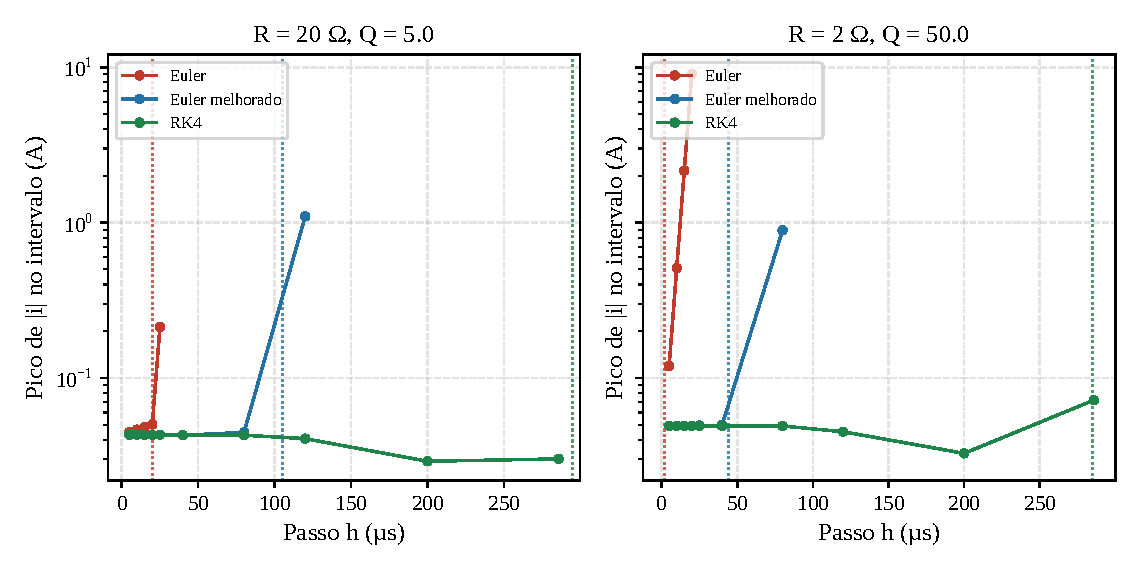
\includegraphics[width=\textwidth]{estabilidade.pdf}
\fonte{Elaborado pelos autores (2026).}
\end{figure}

A integração confirma a teoria: o limite previsto pela função de estabilidade aparece no lugar previsto. Num filtro seletivo, de \(Q\) alto, essa diferença pesa mais que a ordem na escolha do RK4.
